\begin{frame}[t]{Why Graphs} \vspace{4pt}
    \begin{itemize}
        \onslide<1->\item Graphs are a general language for describing and analyzing entities with relations/interactions
        \onslide<2->\item Graphs can model many real life complex knowledge / information / data in expressive way
    \end{itemize}
\end{frame}

\begin{frame}[t]{Graph Examples} \vspace{10pt}
    \only<1>{
        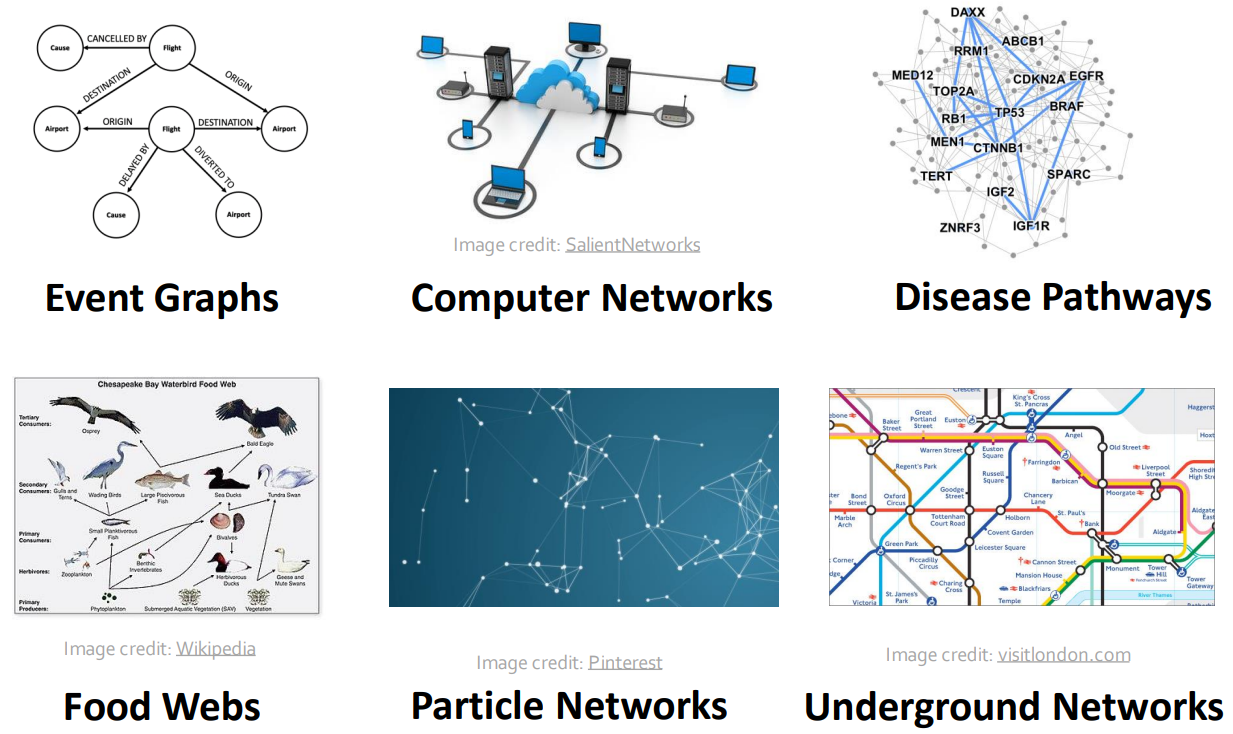
\includegraphics[scale=.35]{graphsOccurances1}
    }
    \only<2>{
        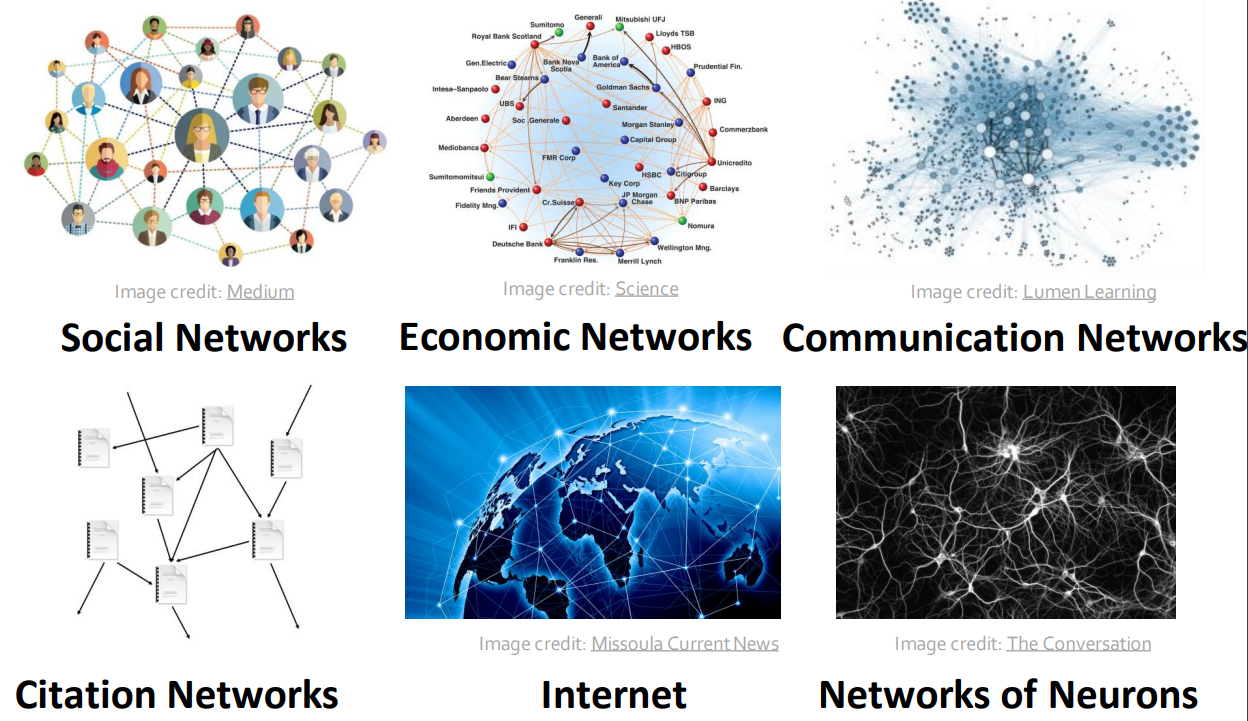
\includegraphics[scale=.33]{graphsOccurances2}
    }
    \only<3>{
        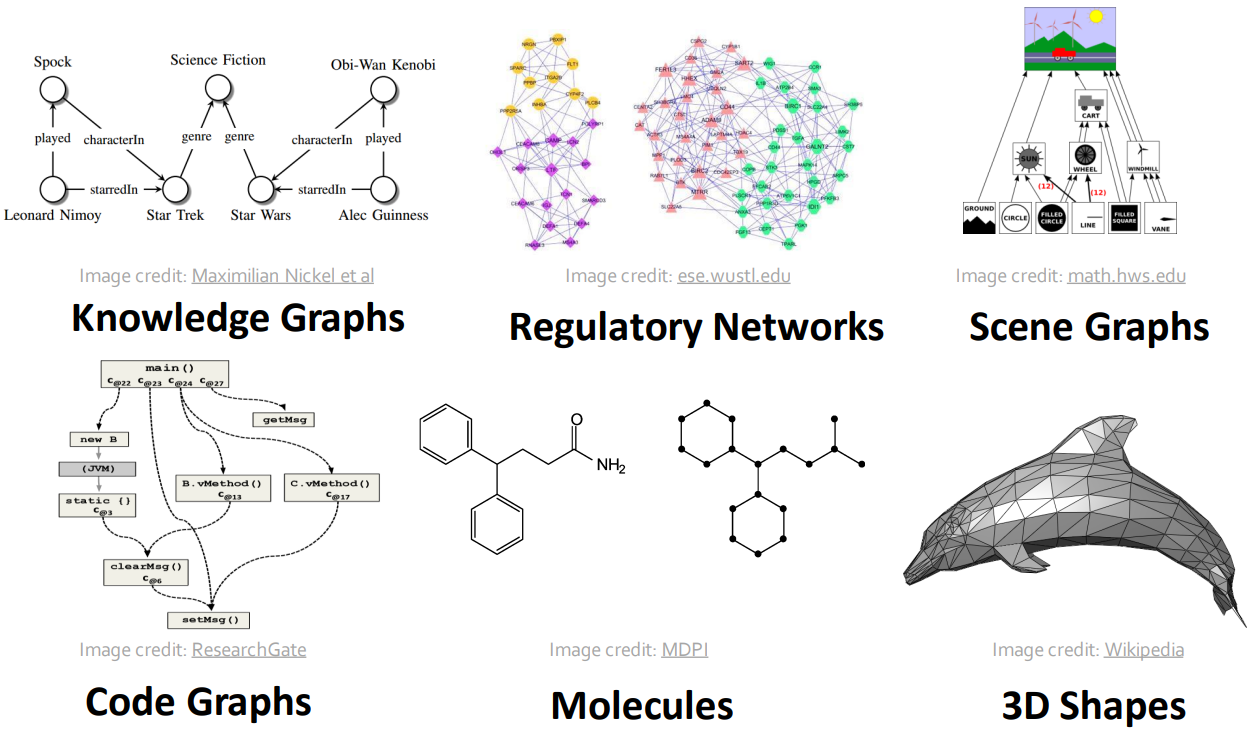
\includegraphics[scale=.35]{graphsOccurances3}
    }
\end{frame}

\begin{frame}[t]{Classic Graph Tasks} \vspace{4pt}
    \only<1>{
        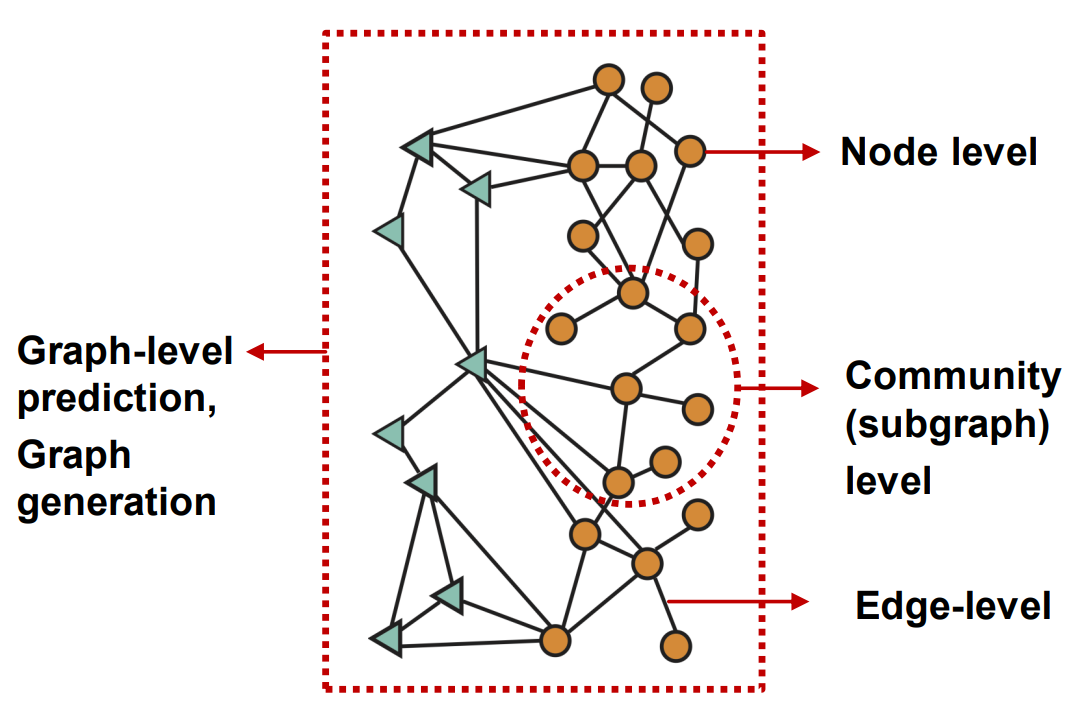
\includegraphics[scale=.35]{classicGraphTasks}
    }
    \only<2>{
        \begin{itemize}
            \item \boldblue{Node classification}: Predict a property of a node\\
                  Example: Categorize online users / items
            \item \boldblue{Link prediction}: Predict whether there are missing links between two nodes\\
                  Example: Knowledge graph completion
            \item \boldblue{Graph classification}: Categorize different graphs\\
                  Example: Molecule property prediction
            \item \boldblue{Clustering}: Detect if nodes form a community\\
                  Example: Social circle detection
            \item \boldblue{Other tasks}:\\
                       Graph generation: Drug discovery\\
                       Graph evolution: Physical simulation
        \end{itemize}
    }
\end{frame}

\begin{frame}[t]{Why is Graph Deep Learning Hard} \vspace{4pt}
    \begin{block}{Networks are complex}
        \begin{itemize}
            \item Arbitrary size and complex topological structure (i.e., no spatial locality like grids)
            \item No fixed node ordering or reference point
            \item Often dynamic and have multimodal features
        \end{itemize}
    \end{block}

    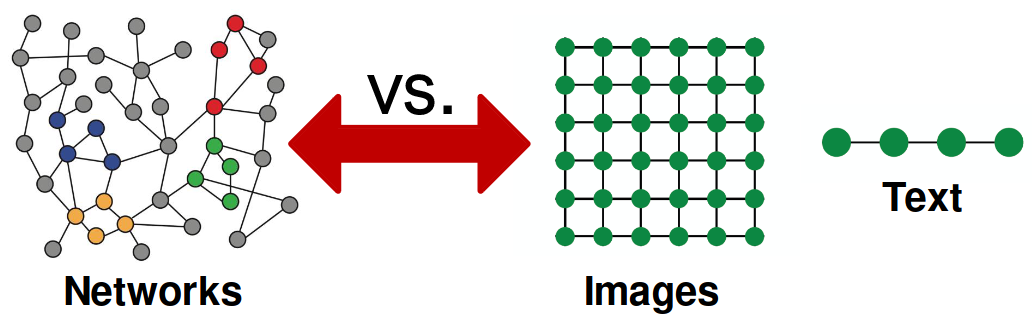
\includegraphics[scale=.3]{networkVsImageAndText}
\end{frame}

\begin{frame}[t]{Traditional Approaches} \vspace{4pt}

    \only<1->{
        \boldblue{Traditional approaches are feature engineering based:}

        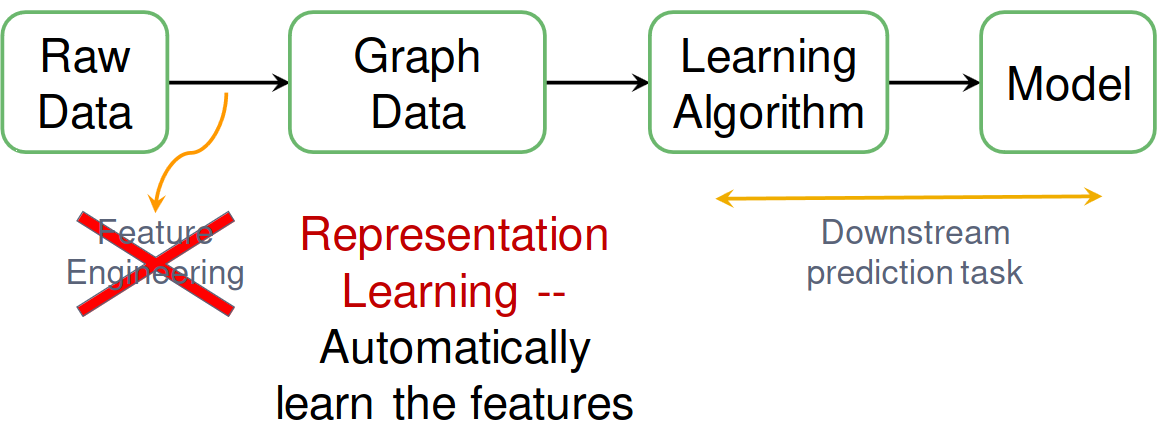
\includegraphics[scale=.27]{traditionalApproaches}
    }
    \only<2>{
        \begin{block}{Feature Extraction}
            Node level, link level, graph level statistical deterministic feature are extracted.
        \end{block}
    }

\end{frame}

